% !TeX root = ../main.tex
\chapter{Dual Statutory Corpus Census and Typology}
\label{app:corpus_census_typology}

This appendix provides the comprehensive census, temporal breakdown, functional typology distribution, and $c\text{-}\mathrm{TF}\text{-}\mathrm{IDF}$ macro domain keyword lexicons for the complete dual statutory corpus comprising 27,096 enactments and 176,421 searchable provisions.

\section{National Statutory Enactment Census (1900--2026)}
\label{sec:app_national_statutory_census}

The national statutory corpus comprises 25,432 enactments cataloged from Lawphil, spanning over a century of Philippine legislative history. Table~\ref{tab:app_national_corpus_breakdown} details the distribution of statutory enactments and extracted provisions across major legislative instruments.

\begin{table}[htbp]
    \centering
    \small
    \caption{National Statutory Corpus Composition across Legislative Classifications}
    \label{tab:app_national_corpus_breakdown}
    \begin{tabular}{llrr}
        \toprule
        \textbf{Statutory Classification} & \textbf{Historical Period} & \textbf{Enactments} & \textbf{Provisions Extracted} \\
        \midrule
        Republic Acts (RA) & 1946--Present & 12,028 & 84,196 \\
        Presidential Decrees (PD) & 1972--1986 & 2,036 & 22,396 \\
        Acts of the Philippine Commission (Act) & 1900--1935 & 4,275 & 21,375 \\
        Executive Orders with Legislative Power (EO) & 1986--1987 & 1,120 & 7,840 \\
        Commonwealth Acts (CA) & 1935--1946 & 733 & 5,131 \\
        Batas Pambansa (BP Blg.) & 1978--1986 & 891 & 4,455 \\
        Letters of Implementation and Orders & Various & 4,349 & 7,316 \\
        \midrule
        \textbf{Total National Statutory Base} & \textbf{1900--2026} & \textbf{25,432} & \textbf{152,709} \\
        \bottomrule
    \end{tabular}
\end{table}

Figure~\ref{fig:app_statute_composition} illustrates the proportional distribution of national enactments across statutory classifications alongside temporal length evolution.

\begin{figure}[htbp]
    \centering
    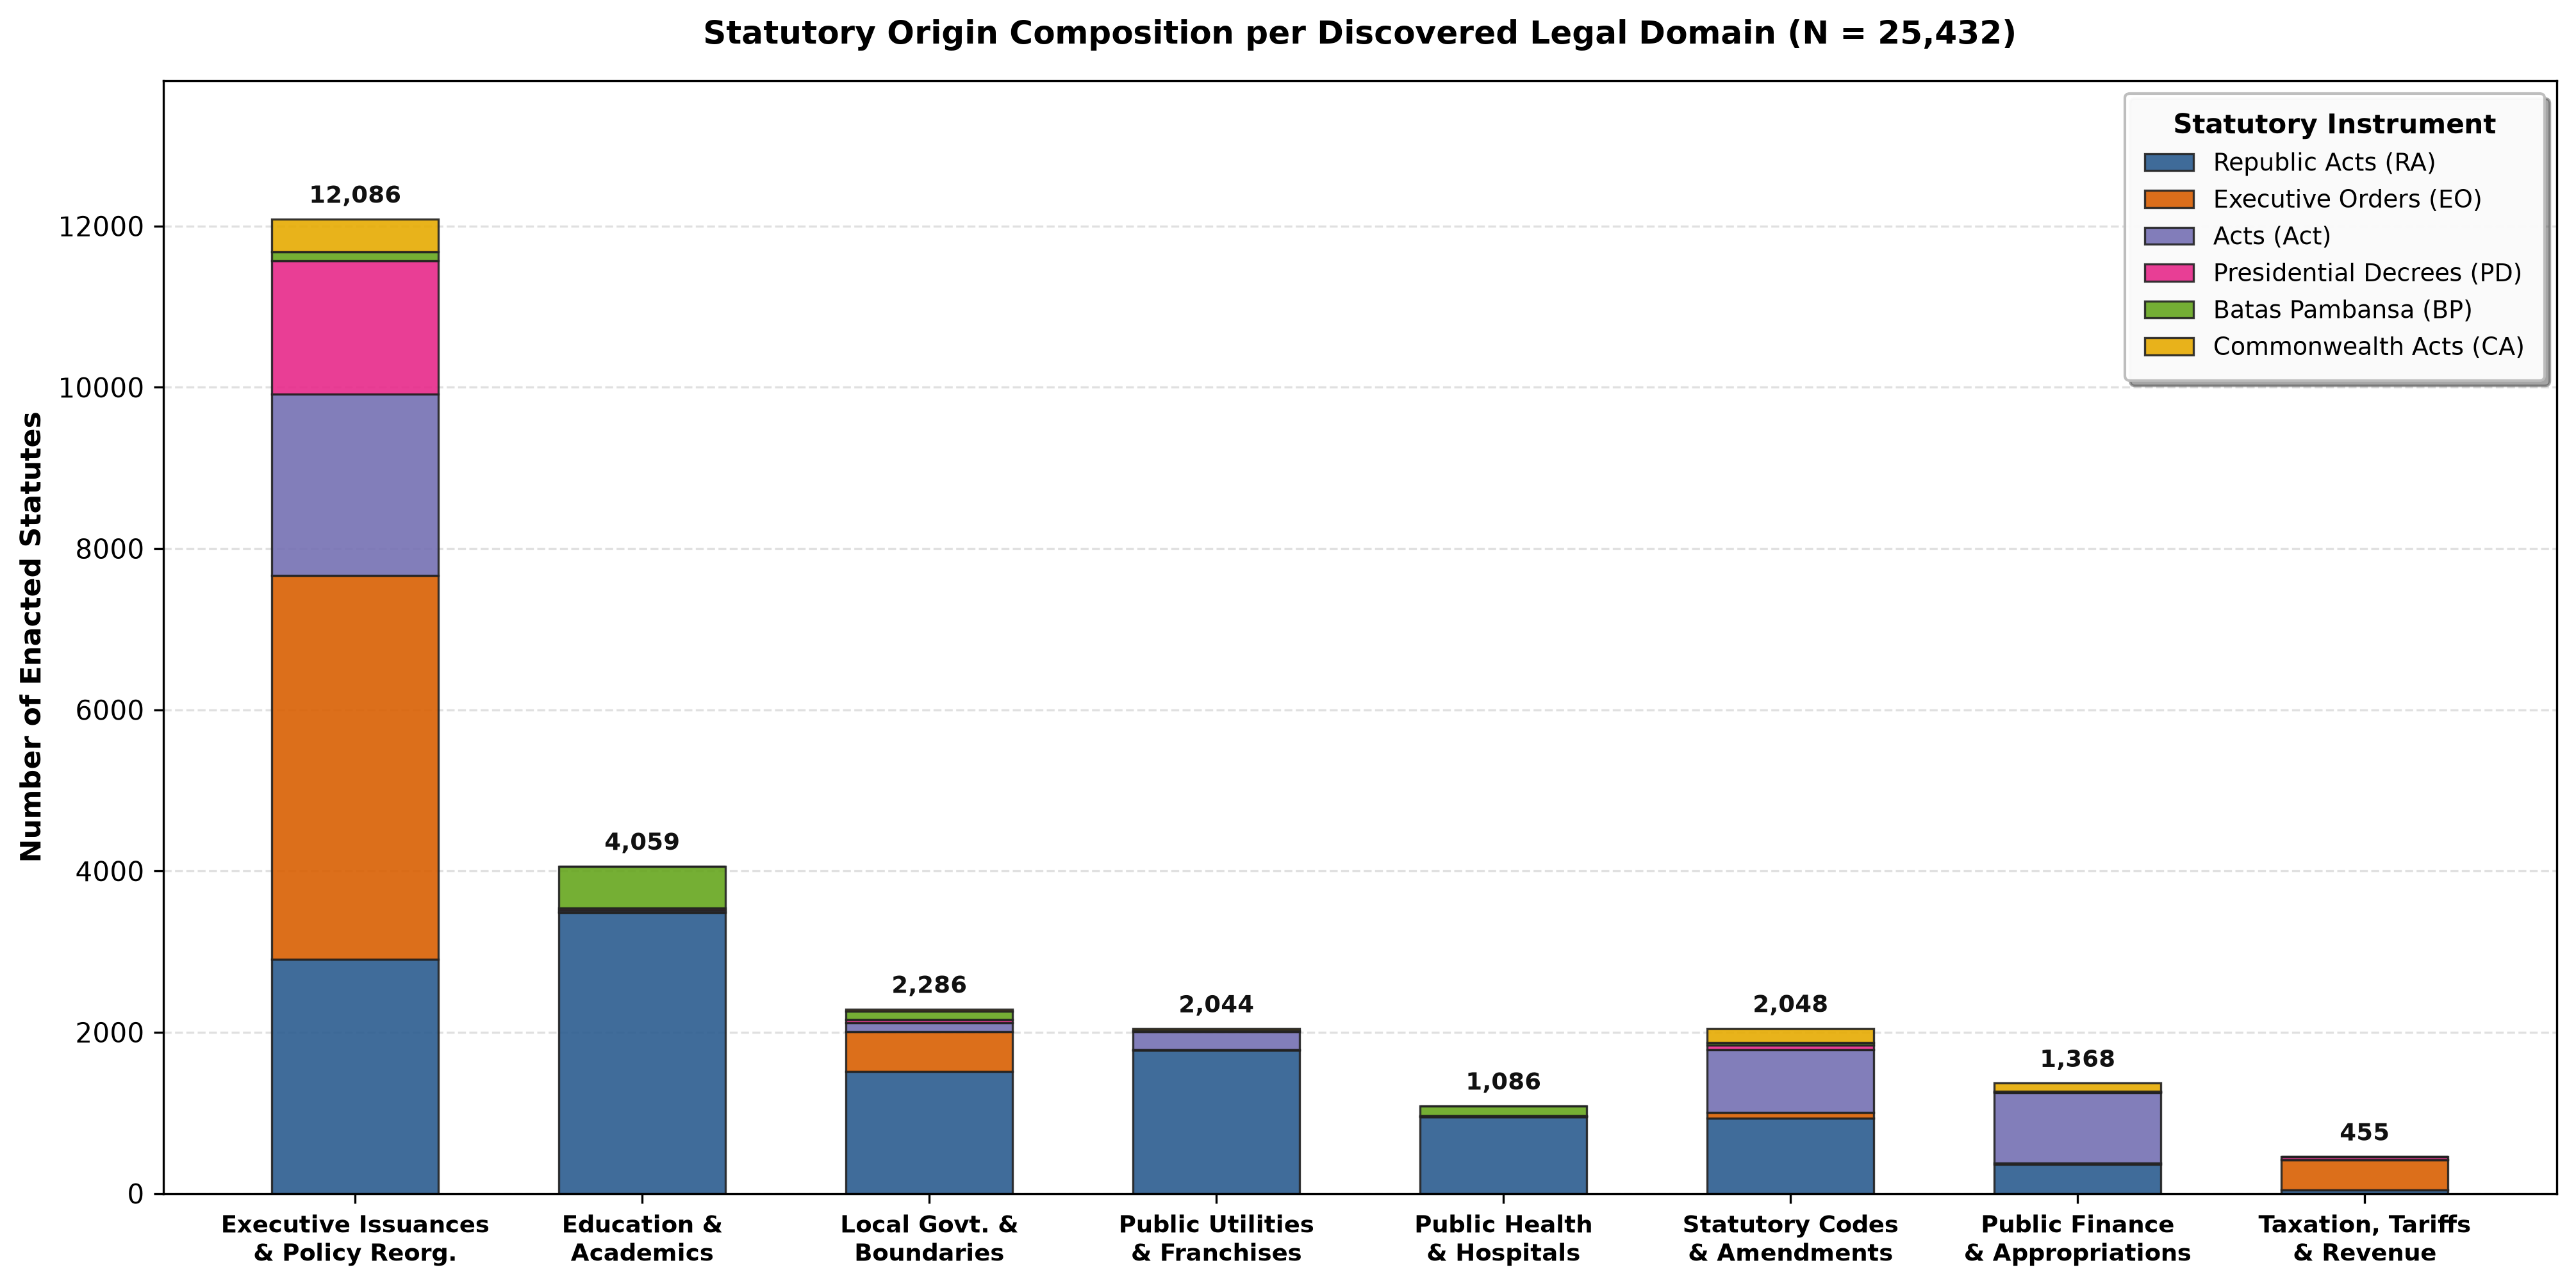
\includegraphics[width=0.82\textwidth]{figs/statute_type_composition.png}
    \caption{Proportional Composition of the National Statutory Knowledge Base ($N = 25,432$ enactments).}
    \label{fig:app_statute_composition}
\end{figure}

\section{Davao City Local Ordinances Census and Typology}
\label{sec:app_davao_ordinance_census}

The local statutory knowledge base encompasses 1,664 digitized Davao City ordinances spanning 1945 to 2026, yielding 23,712 extracted provisions. Table~\ref{tab:app_local_ordinance_eras} summarizes enactment volume across four historical eras.

\begin{table}[htbp]
    \centering
    \small
    \caption{Temporal Distribution of Davao City Local Ordinances}
    \label{tab:app_local_ordinance_eras}
    \begin{tabular}{llcc}
        \toprule
        \textbf{Legislative Era} & \textbf{Historical Governance Context} & \textbf{Ordinances} & \textbf{Provisions Extracted} \\
        \midrule
        Era 1: 1945--1971 & Post-War Rebuilding and City Charter Era & 184 (11.06\%) & 2,116 \\
        Era 2: 1972--1986 & Martial Law and Pre-1987 Constitution & 312 (18.75\%) & 3,962 \\
        Era 3: 1987--2000 & Fifth Republic and 1991 Local Government Code & 468 (28.12\%) & 6,787 \\
        Era 4: 2001--2026 & Modern Digital Legislative Era & 700 (42.07\%) & 10,847 \\
        \midrule
        \textbf{Total Local Ordinance Base} & \textbf{1945--2026} & \textbf{1,664 (100.0\%)} & \textbf{23,712} \\
        \bottomrule
    \end{tabular}
\end{table}

Table~\ref{tab:app_local_typology} partitions the 1,664 ordinances across a six-class functional typology based on substantive subject matter.

\begin{table}[htbp]
    \centering
    \small
    \caption{Six-Class Functional Typology of Davao City Ordinances}
    \label{tab:app_local_typology}
    \begin{tabular}{p{4.5cm}cp{7.5cm}}
        \toprule
        \textbf{Functional Typology Class} & \textbf{Share (\%)} & \textbf{Primary Legislative Scope and Subject Matter} \\
        \midrule
        Revenue and Fiscal Measures & 28.4\% & Local taxation codes, business fees, real property assessments, market stall charges \\
        Public Order, Safety, and Penal & 24.1\% & Curfews, traffic management, speed limits, noise control, public nuisances \\
        Administrative Governance & 19.3\% & Personnel plantilla, office reorganizations, internal Sanggunian rules of procedure \\
        Public Health and Sanitation & 14.8\% & Solid waste segregation, watershed protection, smoking bans, veterinary inspections \\
        Infrastructure and Zoning & 9.2\% & Building setbacks, subdivision approvals, zoning amendments, public works \\
        Social Welfare and Cultural Rights & 4.2\% & Senior citizen privileges, PWD accessibility, Indigenous Peoples ancestral support \\
        \bottomrule
    \end{tabular}
\end{table}

\begin{figure}[htbp]
    \centering
    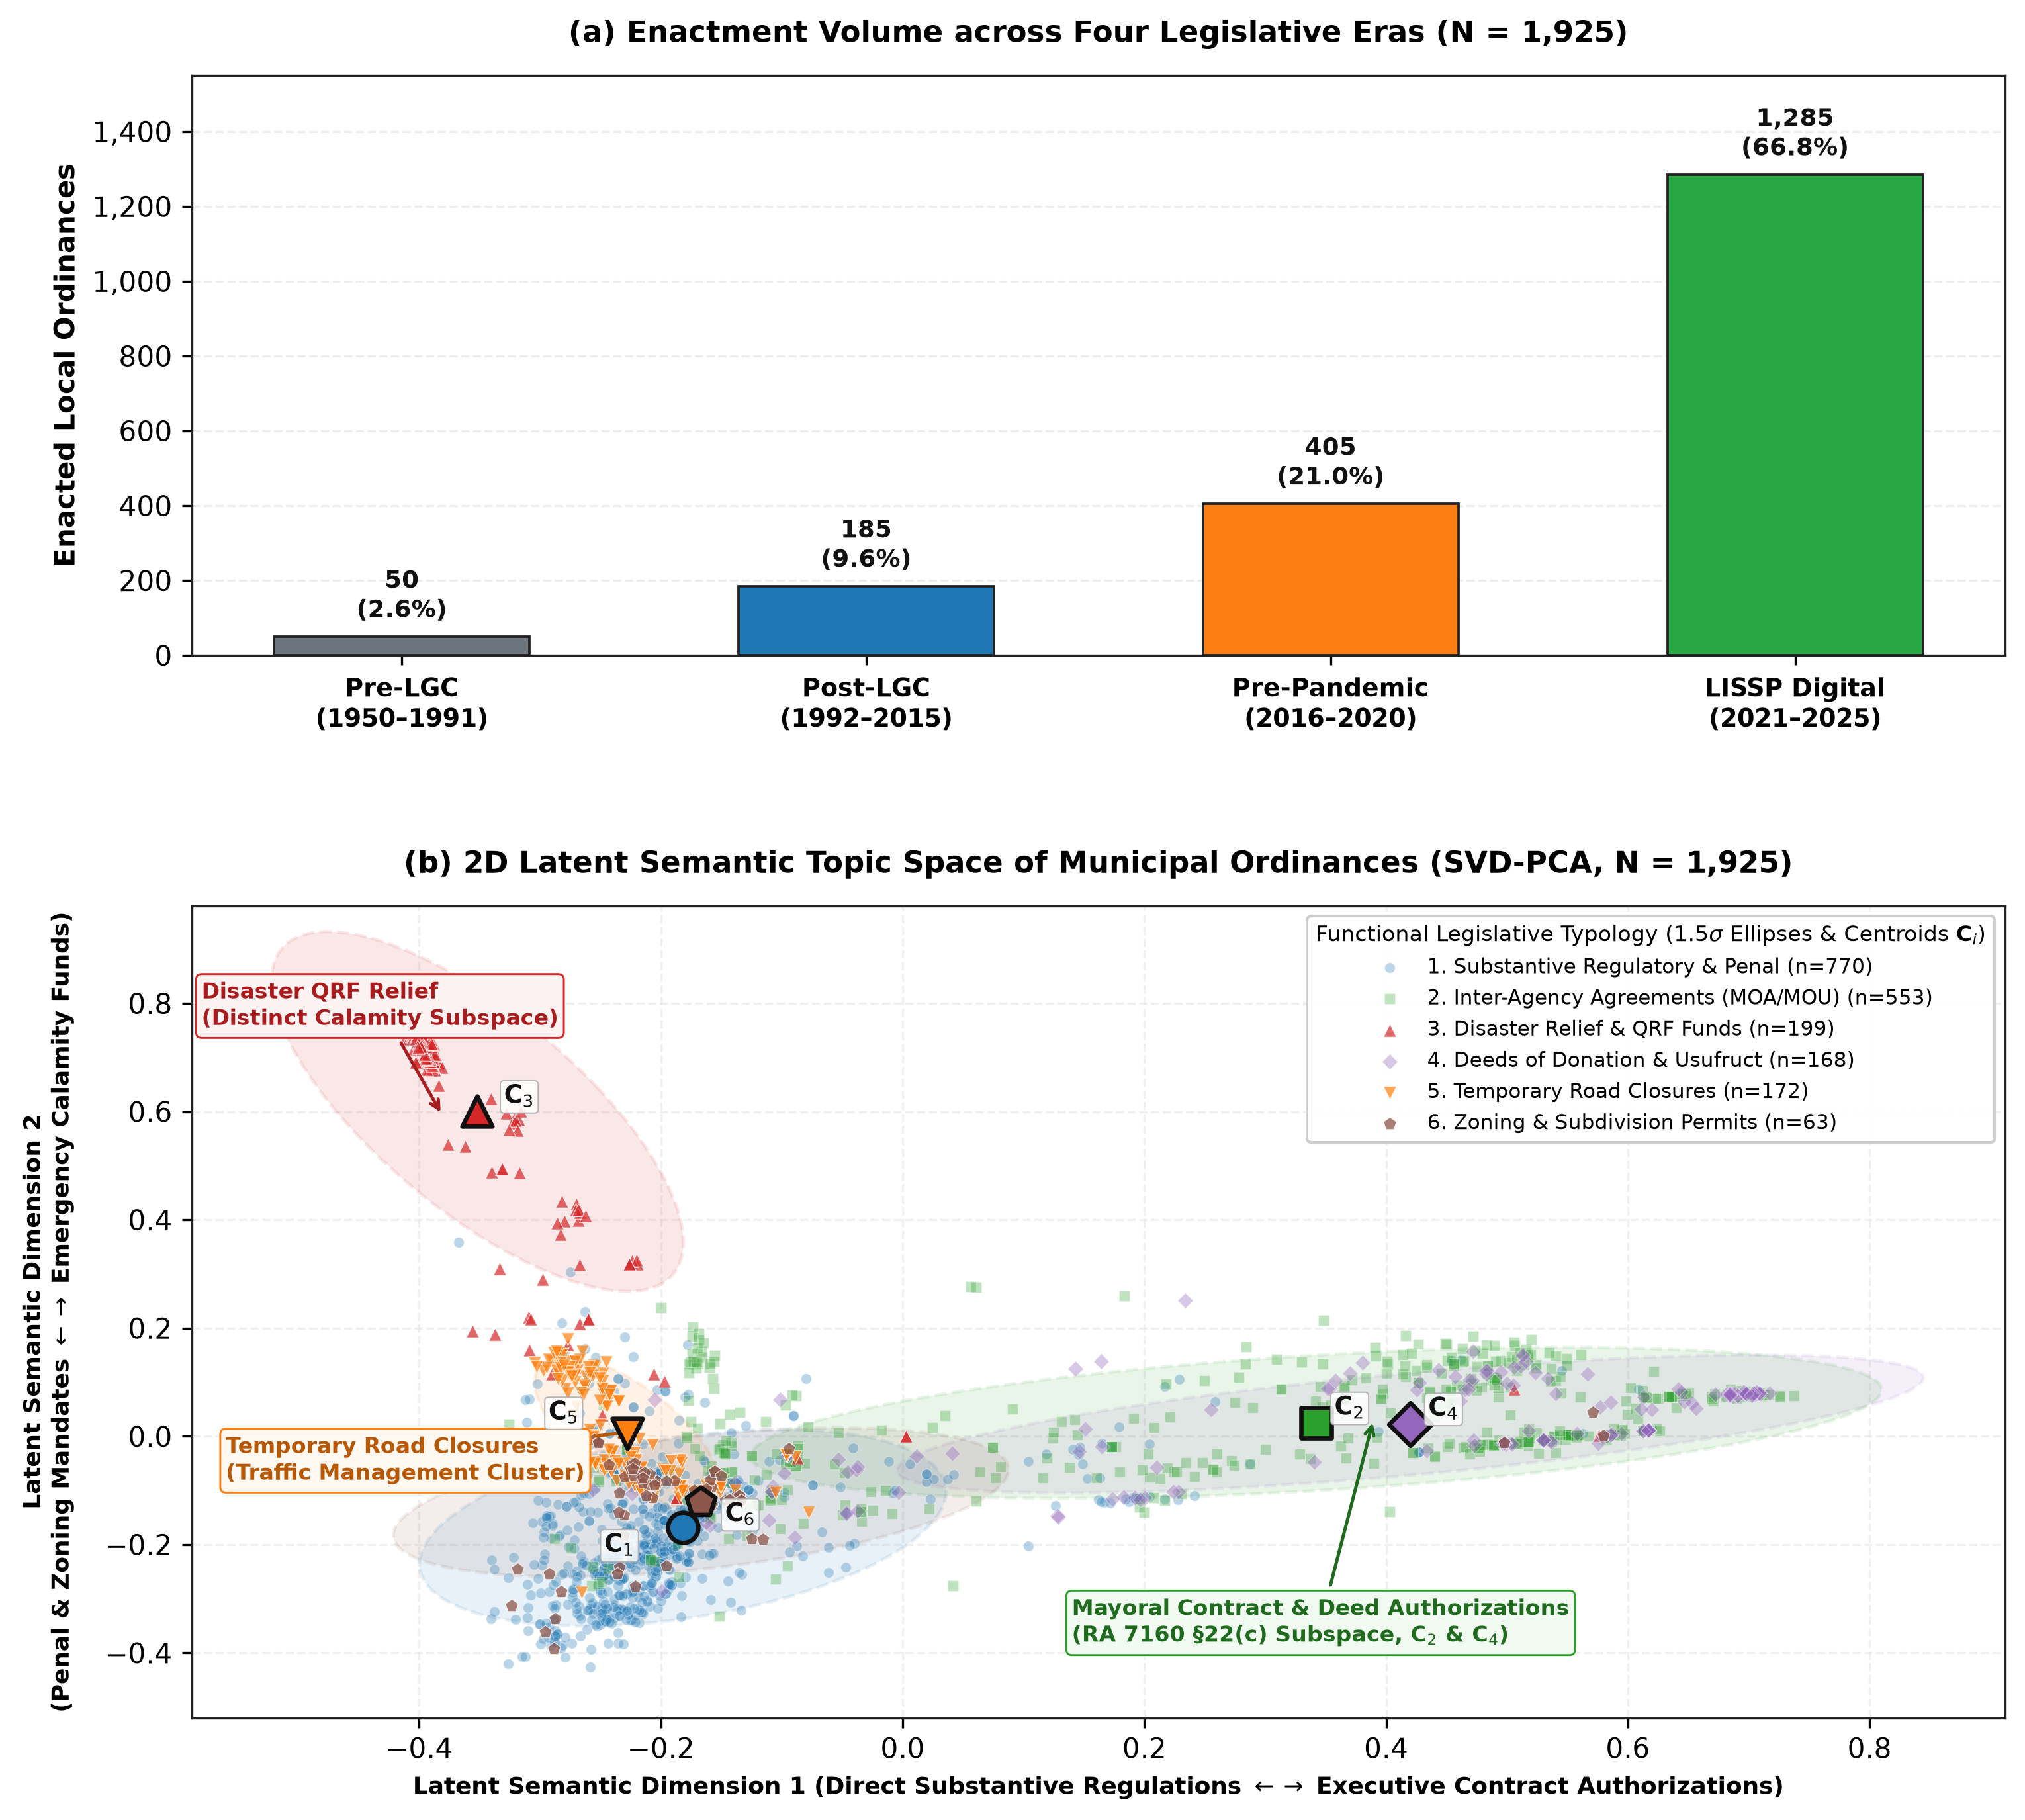
\includegraphics[width=0.85\textwidth]{figs/local_ordinance_temporal_and_typology.png}
    \caption{Temporal Growth and Functional Typology Distribution for Davao City Local Legislation.}
    \label{fig:app_local_temporal_typology}
\end{figure}

\section{Consolidated Macro Legal Domain Dictionaries}
\label{sec:app_macro_domain_dictionaries}

Table~\ref{tab:app_macro_domain_keywords} presents the discriminative keywords identified for the eight macro legal domains extracted via class-based TF-IDF ($c\text{-}\mathrm{TF}\text{-}\mathrm{IDF}$) clustering.

\begin{table}[htbp]
    \centering
    \scriptsize
    \caption{Discriminative Legal Keywords Across Eight Macro Domains ($c\text{-}\mathrm{TF}\text{-}\mathrm{IDF}$)}
    \label{tab:app_macro_domain_keywords}
    \begin{tabular}{lp{12cm}}
        \toprule
        \textbf{Macro Legal Domain} & \textbf{Top Discriminative Legal Keywords and Phrasal Tokens} \\
        \midrule
        1. Administrative Governance & \texttt{sangguniang panlungsod, plantilla, personnel, memorandum, quorum, committee, appointment, tenure, reorganization, civil service, devolved} \\
        \addlinespace
        2. Fiscal and Revenue & \texttt{tax, assessment, schedule of market values, surcharge, fee, collector, gross receipts, amusement tax, real property, delinquent, treasury} \\
        \addlinespace
        3. Penal and Public Order & \texttt{fine, imprisonment, violation, citation, unlawful, misdemeanor, confiscation, summary revocation, curfew, public intoxication, citation ticket} \\
        \addlinespace
        4. Environmental Resources & \texttt{watershed, protected area, ambient air, wastewater, solid waste, segregation, clean water act, timberland, buffer zone, quarry, denr} \\
        \addlinespace
        5. Public Health and Sanitation & \texttt{quarantine, communicable disease, sanitary permit, veterinary, abattoir, immunization, potable water, epidemic, medical clinic, meat inspection} \\
        \addlinespace
        6. Labor and Social Welfare & \texttt{senior citizen, pwd, discount, minimum wage, occupational safety, maternity, day care, informal settler, livelihood, indigenous cultural community} \\
        \addlinespace
        7. Commercial and Trade & \texttt{business permit, mayor's permit, sole proprietorship, corporation, retail trade, price ceiling, weights and measures, fair trade, consumer act} \\
        \addlinespace
        8. Transportation and Infrastructure & \texttt{tricycle franchise, route, public utility vehicle, loading zone, building code, occupancy permit, road right-of-way, terminal, motorized} \\
        \bottomrule
    \end{tabular}
\end{table}

\begin{figure}[htbp]
    \centering
    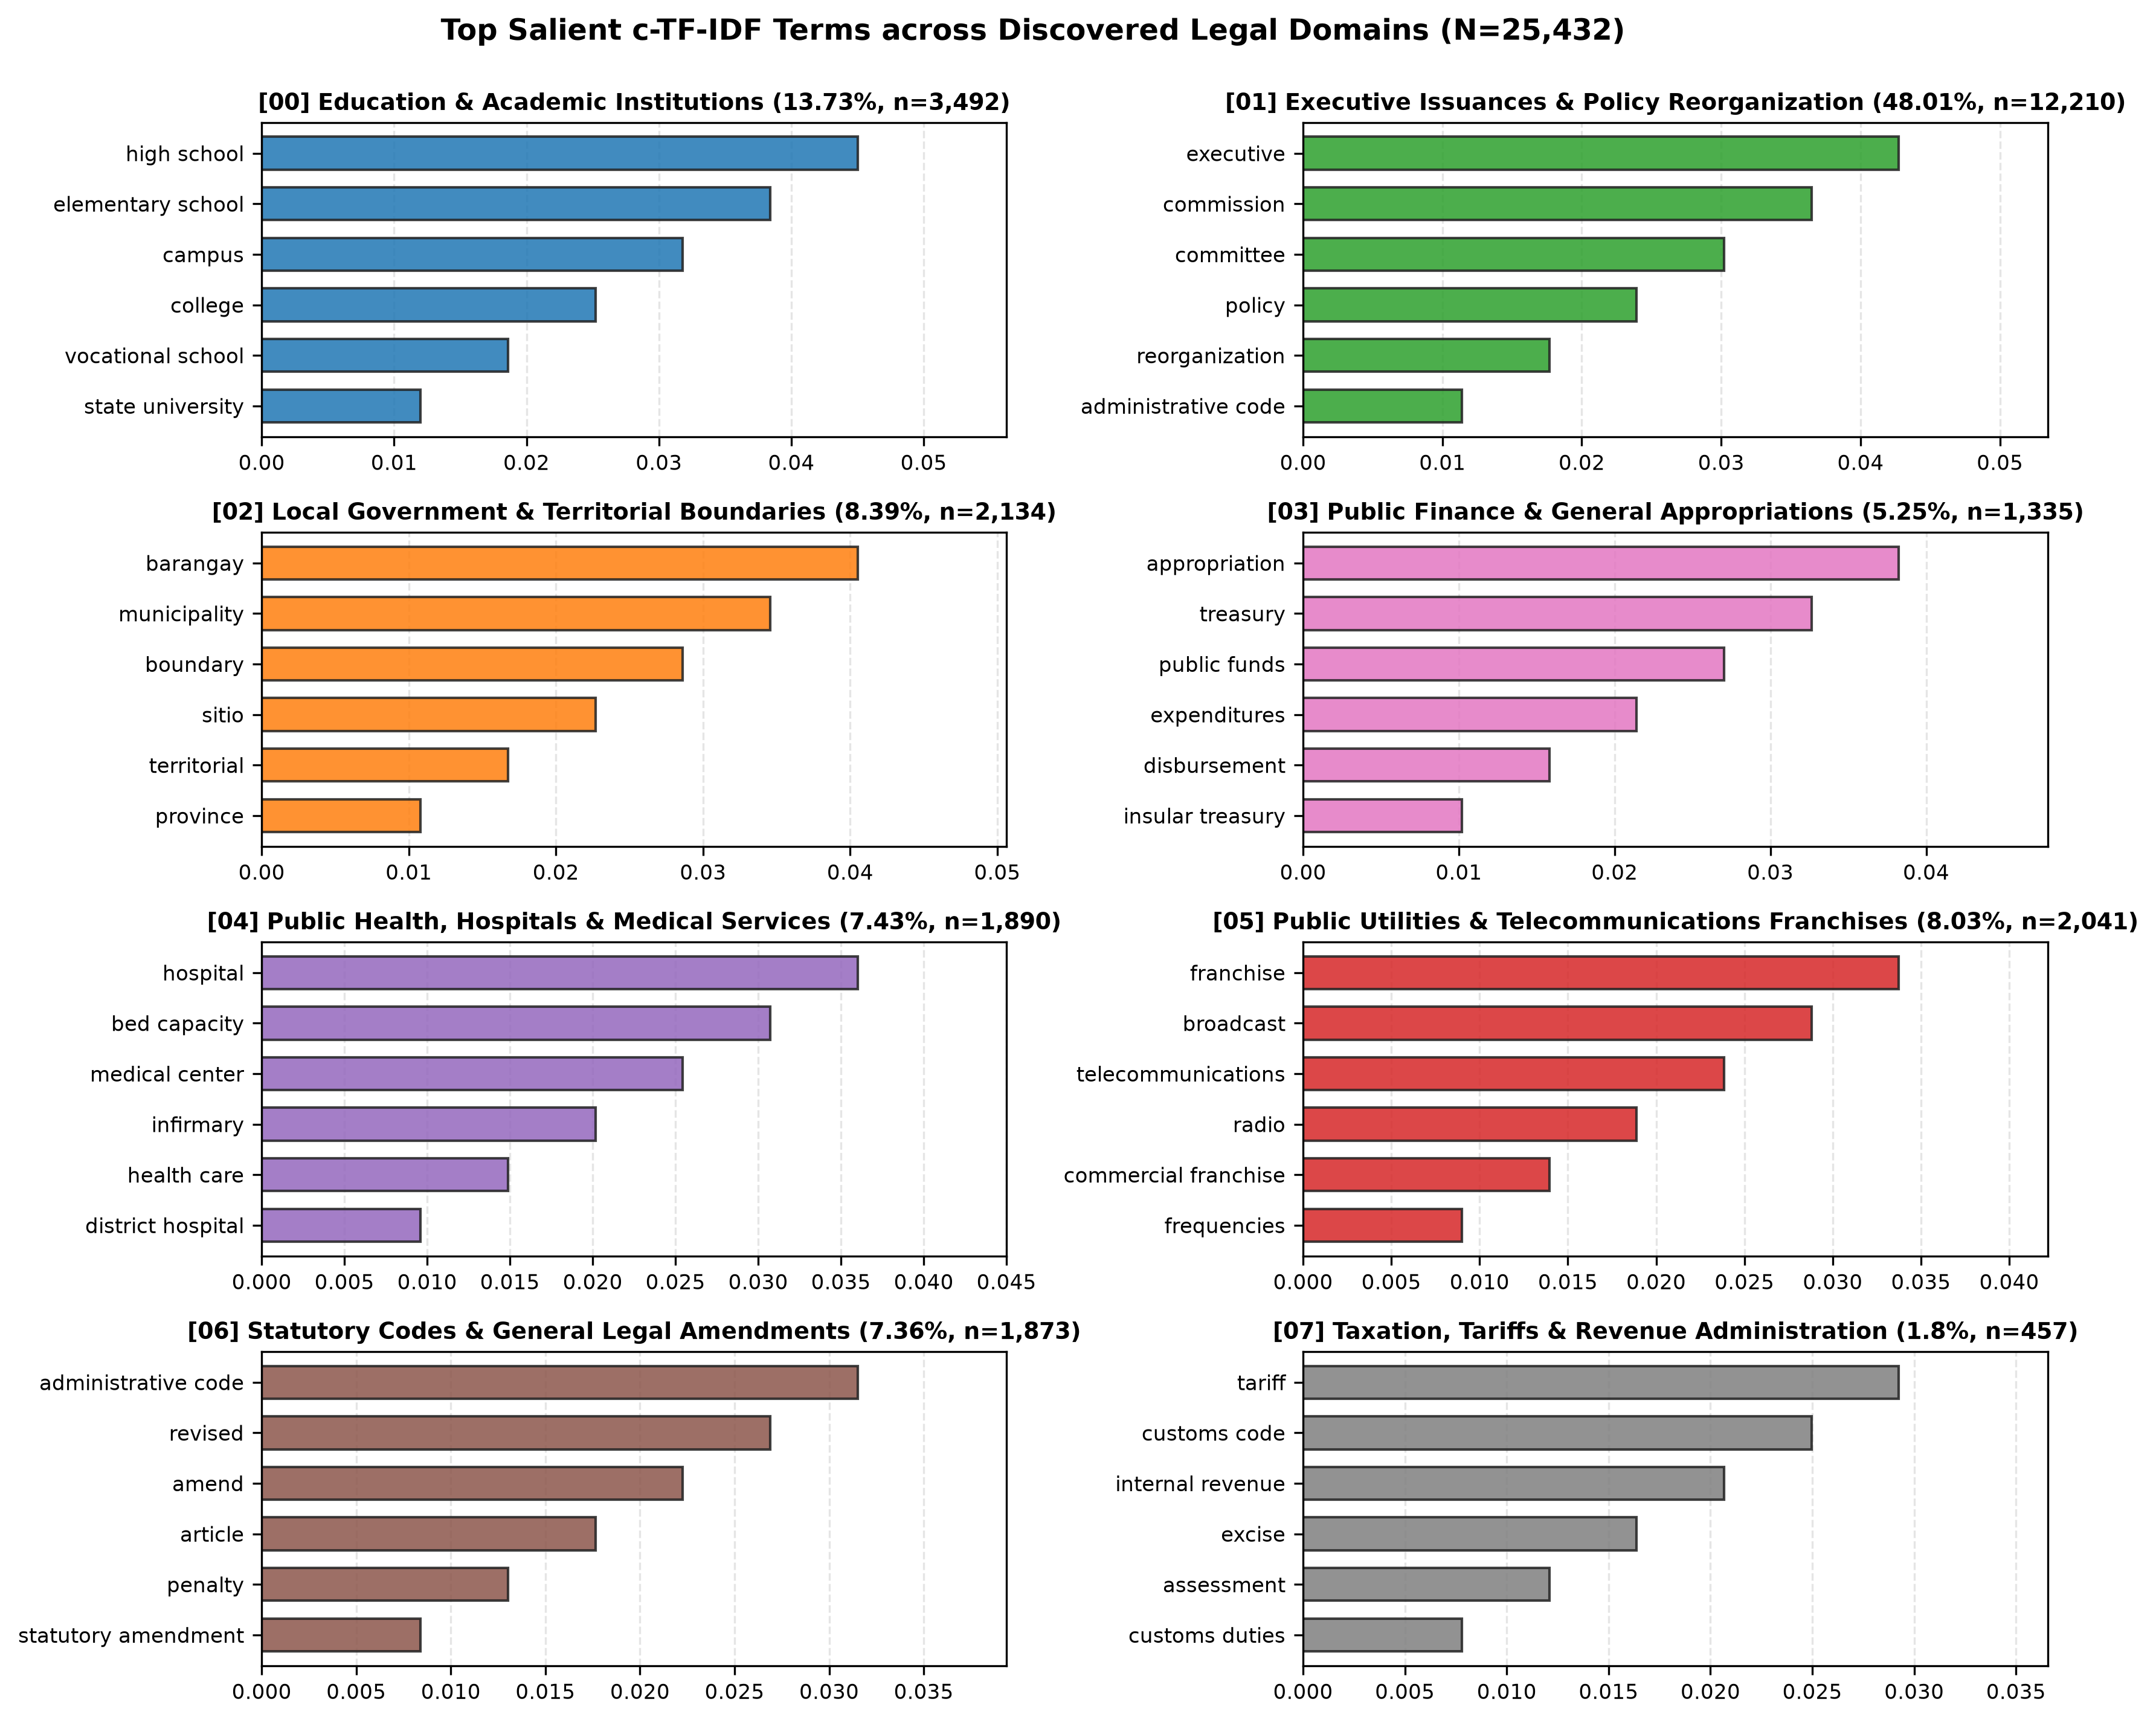
\includegraphics[width=0.88\textwidth]{figs/top_keywords_per_domain.png}
    \caption{Comparative Salience of Discriminative Keywords Across Macro Legal Domains.}
    \label{fig:app_keywords_saliency}
\end{figure}

\section{Provision-Level Token Compliance Distribution}
\label{sec:app_token_length_compliance}

Analysis of the 176,421 searchable provisions demonstrates that \textbf{94.69\% of Davao City ordinance provisions} and \textbf{92.14\% of national statutory provisions} fall strictly within the 512-token sequence limit of modern transformer encoders without requiring destructive textual truncation. The median provision length is 68 tokens, with the 90th percentile reaching 218 tokens.
